\documentclass[11pt, a4paper]{article}

\usepackage{amsmath}
\usepackage[a4paper, margin=1in]{geometry}
\usepackage{amsfonts}
\usepackage{mathtools}

% to insert images
\usepackage{graphicx}
\graphicspath{ {./images/} {../images/}}

% \usepackage{tikz}
% \usetikzlibrary{automata, positioning}

% \usepackage{pgfplots}
% \pgfplotsset{width=5cm,compat=1.9}
\setlength{\parindent}{0em}

\DeclareMathOperator*{\minimize}{minimize}

\begin{document}
    %%%%%%%%%%%%%%%%%%%%%%%%%%%%%%%%%%%%%%%%%%%%%%%%%%%%%%%%%%%%%%%%%%%%%%%%%%%%%%%
    \section{Clustering}
    Clustering is an unsupervised learning techniques that aims to finds clusters or groups in the data such that observations in the same group are similar to each other while observations in different groups are different from each other.\newline

    Clustering is useful for an exploratory analysis of the data and also useful in problems like customer segmentation.

    %%%%%%%%%%%%%%%%%%%%%%%%%%%%%%%%%%%
    \subsection{K-means Clustering}
    A very powerful technique that organizes the data into $K$ distinct groups such that each observation will fall into exactly one group and when all the groups are combined, they cover the entire data set. $K$ is determined beforehand and is the number of clusters we are going to make.\newline

    The fundamental idea of clustering is to reduce the within cluster variation. Let $C_{k}$ denote the set containing the indices of the points falling in the cluster $k$ and $W(C_{k})$ be the within cluster variation for cluster $k$. Then,
    \begin{align*}
        \minimize_{C_{1},\ldots,C_{K}} \sum_{k=1}^{K} W(C_{k})
    \end{align*}

    Using Euclidean distance as a measure of the intercluster distance between two points, we can redefine the optimization summing across all the dimensions of the data as
    \begin{align*}
        \minimize_{C_{1},\ldots,C_{K}} \sum_{k=1}^{K} \frac{1}{\vert C_{k} \vert} \bigg\{\sum_{i_{1}, i_{2} \in C_{k}} \sum_{j=1}^{p} (x_{i_{1}j} - x_{i_{2}j})^{2} \bigg \}
    \end{align*}
    where $\vert C_{k} \vert$ is the number of observations in the cluster $C_{k}$. Considering all possible partitions is impossible for large $n$ and we use the following algorithm to obtain the local optimum.


    %%%%%%%%%%%%%%%%%%%%%%%%%%%%%%%%%%%
    \subsubsection{Algorithm}
    We repeat the following until some predefined convergence criteria
    \begin{enumerate}
        \item Random assign a cluster in $1, \ldots, K$ to each observation in the data.
        \item Repeat the following till convergence
        \begin{enumerate}
            \item Calculate the centroid for each cluster where centroid is a $p$ dimensional vector whose each component is the average of the components of all the points that fall in the considered cluster.
            \item Assign each observation the cluster index of the centroid that is closest to the given observation (using Euclidean distance).
        \end{enumerate}
    \end{enumerate}

    \textbf{It is usually a good idea to center and standardize the variables first} so that the individual magnitudes and variances don't affect the Euclidean distances drastically.

    To see why using distance from centroid is a good replacement for the pairwise distance, consider the following equation
    \begin{align*}
        \sum_{i_{1}, i_{2} \in C_{k}} (x_{i_{1}} - x_{i_{2}})^{T} (x_{i_{1}} - x_{i_{2}}) = \frac{1}{2} \sum_{i \in C_{k}} \sum_{j \in C_{k}} (x_{i} - x_{j})^{T}(x_{i} - x_{j})
    \end{align*}
    where the right side allows for all possible pairs including the ones where the indices might repeat. Continuing to expand the right hand side,
    \begin{align*}
        \sum_{i \in C_{k}} \sum_{j \in C_{k}} (x_{i} - x_{j})^{T}(x_{i} - x_{j}) &= \sum_{i \in C_{k}} \bigg(\vert C_{k} \vert (x_{i}^{T} x_{i}) - 2x_{i}^{T} \sum_{j \in C_{k}} x_{j} + \sum_{j \in C_{k}} x_{j}^{T} x_{j} \bigg)\\
        &= \sum_{i \in C_{k}} \bigg( \vert C_{k} \vert (x_{i}^{T} x_{i}) - 2\vert C_{k} \vert x_{i}^{T} \bar{x} + \sum_{j \in C_{k}} x_{j}^{T} x_{j} \bigg)\\
        &= \sum_{i \in C_{k}} \bigg( \vert C_{k} \vert (x_{i}^{T} x_{i}) - 2\vert C_{k} \vert x_{i}^{T} \bar{x} \bigg) + \sum_{i \in C_{k}} \vert C_{k} \vert x_{i}^{T} x_{i}\\
        &= \sum_{i \in C_{k}} \bigg( 2\vert C_{k} \vert (x_{i}^{T} x_{i}) - 2\vert C_{k} \vert x_{i}^{T} \bar{x} \bigg)\\
        &= 2 \vert C_{k} \vert \bigg\{ \bigg( \sum_{i \in C_{k}}  (x_{i}^{T} x_{i}) \bigg) - \vert C_{k} \vert \bar{x}^{T} \bar{x} \bigg\}\\
        &= 2 \vert C_{k} \vert \bigg\{ \bigg( \sum_{i \in C_{k}}  (x_{i}^{T} x_{i}) \bigg) - 2\vert C_{k} \vert \bar{x}^{T} \bar{x} + \vert C_{k} \vert \bar{x}^{T} \bar{x} \bigg\}\\
        &= 2 \vert C_{k} \vert \bigg\{ \bigg( \sum_{i \in C_{k}}  (x_{i}^{T} x_{i}) \bigg) - 2 (\sum_{i \in C_{k}} x_{i}^{T} \bar{x}) + \vert C_{k} \vert \bar{x}^{T} \bar{x} \bigg\}\\
        &= 2 \vert C_{k} \vert \bigg\{ \sum_{i \in C_{k}}  x_{i}^{T} x_{i} - 2 x_{i}^{T} \bar{x} + \bar{x}^{T} \bar{x} \bigg\}\\
        &= 2 \vert C_{k} \vert \bigg\{ \sum_{i \in C_{k}}  (x_{i} - \bar{x})^{T} (x_{i} - \bar{x}) \bigg\}\\
        \text{Thus, } \frac{1}{\vert C_{k} \vert} \bigg\{\sum_{i_{1}, i_{2} \in C_{k}} \sum_{j=1}^{p} (x_{i_{1}j} - x_{i_{2}j})^{2} \bigg \} &= \bigg\{ \sum_{i \in C_{k}}  (x_{i} - \bar{x})^{T} (x_{i} - \bar{x}) \bigg\}
    \end{align*}

    Thus, the quantity we set out to minimize for each cluster is indeed the sum of distance of each point from the centroid of the cluster, which means the cluster is to be chosen based on the closest centroid to minimize the overall intra cluster distance.\newline

    \textbf{The optimum found by K-means clustering is local which makes it important to run the algorithm with different random initializations to get the minima}.\newline

    \textbf{Elbow Curve} is a plot between the total intra cluster distance vs the number of cluster $K$ and is a visual method to obtain the optimum number of clusters to use. The elbow shape refers to the fact that if there is indeed clusters present in the data, the plot will see a sharp decline in the intra cluster distance for some $k$.\newline
    Note that the curve is going to always keep decreasing as in the limiting case when we have $n$ points and $n$ clusters, the total distance will be zero. Hence, the number of clusters must be carefully chosen.


    %%%%%%%%%%%%%%%%%%%%%%%%%%%%%%%%%%%
    \subsection{Hierarchical Clustering}
    $K$-means suffers from the disadvantage that the number of clusters needs to be specified beforehand. Hierarchical does not require such a consideration beforehand. here we dicsuss the \textbf{bottom-up} or \textbf{agglomerative clustering} approach. Hierarchical clustering is visualized using a \textbf{dendogram} which is a tree like diagram draw upside down. Starting from the bottom, branches are originate from the individual data points and slowly start merging as we move upward. The earlier the branches merge, the similar the data points are and vice versa. (Be careful to not judge the similarity from the proximity on the horizontal axis)\newline

    \begin{figure}[h]
    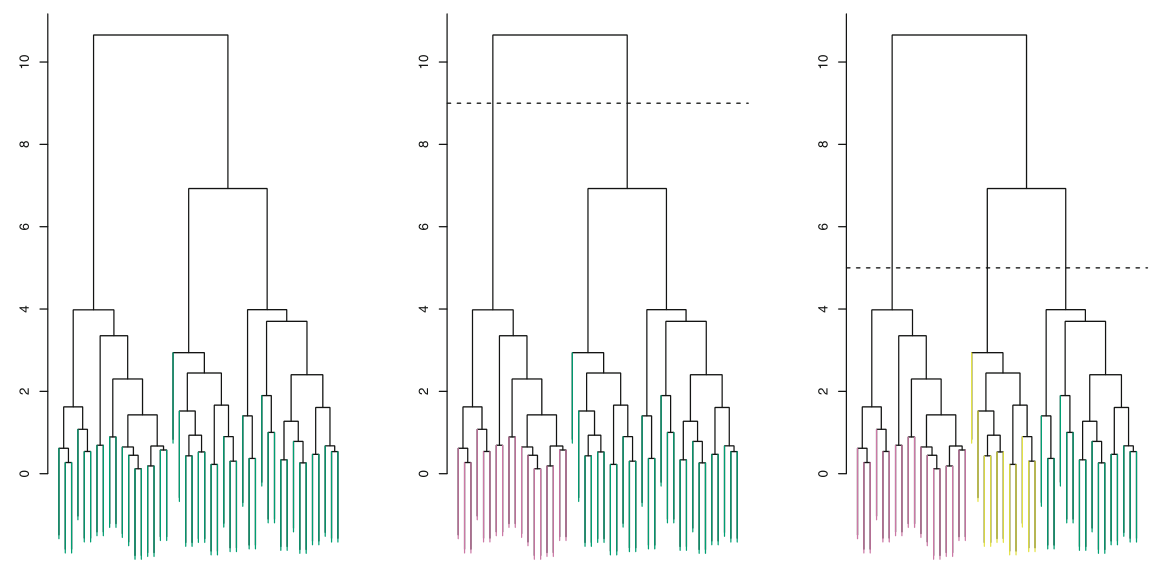
\includegraphics[scale=0.5]{dendogram}
    \centering
    \caption{Visualization of dendogram. The two curves on the right colour the different clusters obtained based on the height at which we decide to cut.}
    \label{fig:dendogram} %\ref{fig:dendogram}
    \end{figure}

    The number of clusters is simply determined by the height at which we made the cut. The middle figure in figure \ref{fig:dendogram} shows a cut at height 9 which results in two branches and thus two clusters.\newline
    Changing the height from the highest value to the lowest value will result in 1 and $n$ clusters respectively. Thus, we do not need to specify the number of clusters beforehand but it is rather to be chosen by us based on the height. This height can be seen similar to $K$ in $K$-means clustering.\newline

    The inherent nesting of the clusters as indicated visually by the dendogram may not be possible in every data set and there will be cases when $K$-means clustering may be superior.


    %%%%%%%%%%%%%%%%%%%%%%%%%%%%%%%%%%%
    \subsubsection{Algorithm}
    Hierarchical Clustering is performed in a bottom-up approach. Start with $n$ clusters where each observation is it's own cluster. Define a dissimilarity measure between each pair of observation. This can be Euclidean distance as well. Now, cluster the observations that are least dissimilar into the same group, which will give us $n-1$ clusters. Again use the dissimilarity measure to group two similar observations until the total number of clusters is 1.\newline

    Consequently, there will be cases when we need to determine the dissimilarity between a group and an observation or a pair of groups. This is done using \textbf{linkage}. Four types of linkages used are \textbf{complete, average, single} and \textbf{centroid}. Average and complete linkages are preferred over single linkages, and all three are more popular than centroid linkage. Average and complete likages will usually give balanced dendograms.\newline

    Following are teh descriptions of individual types of linkages
    \begin{itemize}
         \item Complete\newline
         Maximal intercluster dissimilarity. Take the maximum of the pairwise dissimilarity between observations of cluster A and cluster B.
         \item Single\newline
         Minimum intercluster dissimilarity. Take the minimum of the pairwise dissimilarity between observations of cluster A and cluster B.\newline
         Single linkage can result in extended trailing clusters in which single observations fuse one at a time.
         \item Average\newline
         Mean intercluster dissimilarity. Take the average of the pairwise dissimilarity between observations of cluster A and B.
         \item Centroid\newline
         Take the dissimilarity between the centroid of cluster A and B. Centroid linkages can result in undesirable inversions.
    \end{itemize}


    \begin{figure}[h]
    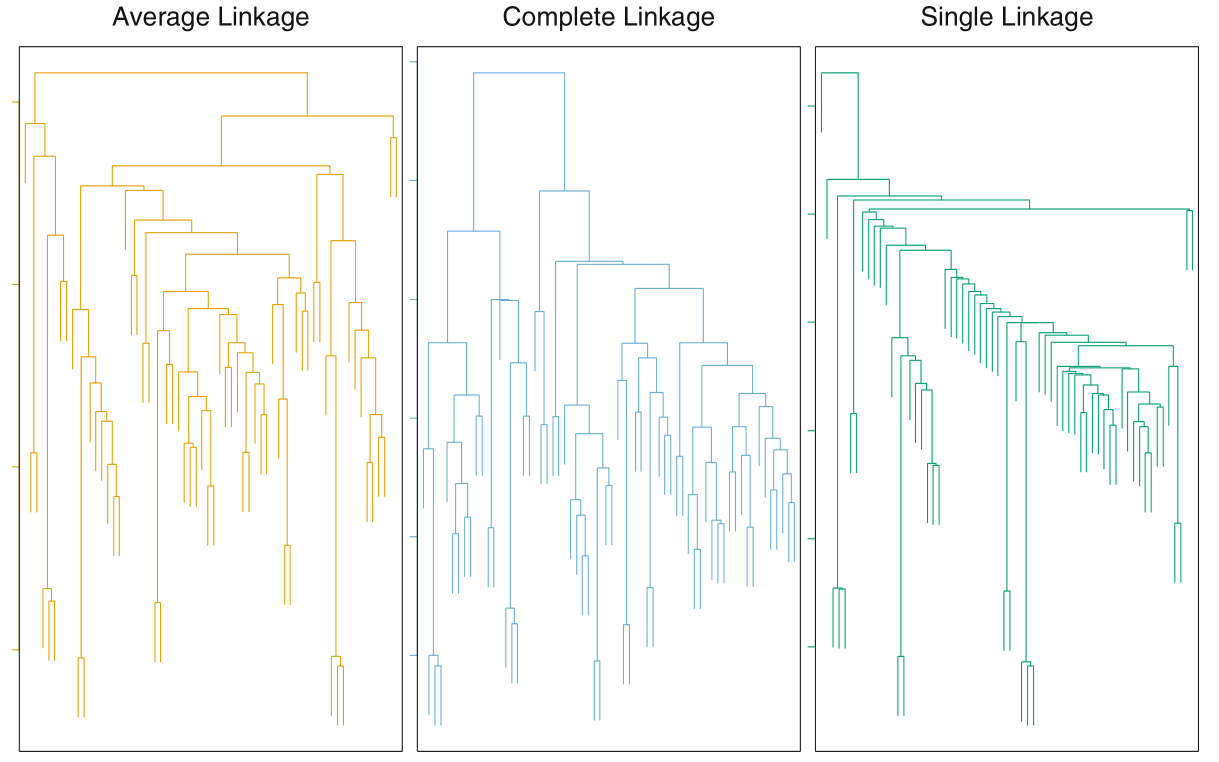
\includegraphics[scale=0.5]{dendogram_linkages}
    \centering
    \caption{Visualization of dendograms obtained for different choice of linkages.}
    \label{fig:dendogram_linkages} %\ref{fig:dendogram_linkages}
    \end{figure}

    The algorithm can be summarized as follows
    \begin{enumerate}
        \item Start with $n$ clusters where each observation is it's own cluster. Compute $n(n-1)/2$ pairwise dissimilarity measures between all pairs.
        \item For $i=n, n-1, \ldots, 2$
        \begin{enumerate}
            \item Compute the pairwise dissimilarity between all $i$ clusters and take the two clusters with the least dissimilarity (or highest similarity). Fuse them into a single cluster. The dissimilarity measure is also indicative of the height in the dendogram where the two clusters fuse.
            \item Recompute the pairwise dissimilarity between the $n-1$ clusters.
        \end{enumerate}
    \end{enumerate}


    %%%%%%%%%%%%%%%%%%%%%%%%%%%%%%%%%%%
    \subsubsection{Dissimilarity Measures}
    So far, euclidean distance has been considered as the defacto dissimilarity measure. In some cases, this may not work well if the magnitude of the observations vary significantly between the different predictors. In such cases, correlation based measures can be preferred since they will group observations with similar behaviour together and not focus on magnitude.\newline
    This can be useful in retail behaviour when we want to check profiles based on the whether similar products are purchased rather than how many of them are purchased.


    %%%%%%%%%%%%%%%%%%%%%%%%%%%%%%%%%%%
    \subsubsection{Key Considerations}
    Following are a set of general rules when doing clustering
    \begin{itemize}
        \item centering and bringing the variables to the same scale is useful when measuring Euclidean distance for the obvious reason of not letting magnitudes affect the distances.
        \item Different types of clustering approaches should be explored to check which performs the best. This is important as in unsupervised learning, the structure of data is not known beforehand and it is important to explore multiple hypothesis.
        \item Several choices of similarity measures and linkages can be explored for further understanding of data.
        \item Clustering can be non robust and thus the results should be "validated" by performing clustering on multiple subsets of data to assure stability.
        \item In come cases, the hard cluster assignment of $K$-means and hierarchical clustering may not be useful. Probabilistic models like mixture models can be explored in this case.
    \end{itemize}
\end{document}